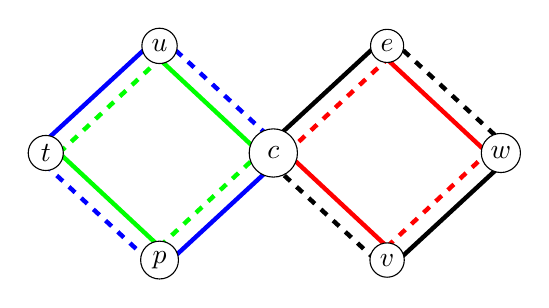
\begin{tikzpicture}[scale=1.7]
\draw[ultra thick, dashed, green] (0,0) -- (0.75,.7);
\draw[ultra thick, green] (0.75,.7) -- (1.5,0);
\draw[ultra thick, green] (0,0) -- (0.75,-.7);
\draw[ultra thick, dashed, green] (0.75,-.7) -- (1.5,0);
\draw[ultra thick, blue] (-0.2,0) -- (0.72,.85);
\draw[ultra thick, dashed, blue] (0.78,.85) -- (1.7,0);
\draw[ultra thick, dashed, blue] (-.2,0) -- (0.72,-.85);
\draw[ultra thick, blue] (0.78,-.85) -- (1.7,0);
\node[circle, fill=white, draw=black, text=black, inner sep=2pt] at (-.1,0) {$t$}; 
\node[circle, fill=white, draw=black, text=black,  inner sep=2pt] at (0.75,-.8) {$p$}; 
\node[circle, fill=white, draw=black, text=black,  inner sep=2pt] at (0.75,.8) {$u$};

\begin{scope}[shift={(1.7,0)}]
\draw[ultra thick, dashed, red] (0,0) -- (0.75,.7);
\draw[ultra thick, red] (0.75,.7) -- (1.5,0);
\draw[ultra thick, red] (0,0) -- (0.75,-.7);
\draw[ultra thick, dashed, red] (0.75,-.7) -- (1.5,0);
\draw[ultra thick, black] (-0.2,0) -- (0.72,.85);
\draw[ultra thick, dashed, black] (0.78,.85) -- (1.7,0);
\draw[ultra thick, dashed, black] (-.2,0) -- (0.72,-.85);
\draw[ultra thick, black] (0.78,-.85) -- (1.7,0);
\node[circle, fill=white, draw=black, text=black, inner sep=4pt] at (-.1,0) {$c$}; 
\node[circle, fill=white, draw=black, text=black,  inner sep=2pt] at (1.6,0) {$w$}; 
\node[circle, fill=white, draw=black, text=black,  inner sep=2pt] at (0.75,-.8) {$v$}; 
\node[circle, fill=white, draw=black, text=black,  inner sep=2pt] at (0.75,.8) {$e$};
\end{scope}
\end{tikzpicture}
